%% GarudaChip --- IEEE conference paper (IEEEtran) with native TikZ figures.
%% Build: pdflatex garudachip_paper ; pdflatex garudachip_paper
\documentclass[conference]{IEEEtran}
\IEEEoverridecommandlockouts
\usepackage{cite}
\usepackage{amsmath,amssymb,amsfonts}
\usepackage{graphicx}
\usepackage{textcomp}
\usepackage{xcolor}
\usepackage{booktabs}
\usepackage[hidelinks]{hyperref}
\usepackage{url}
\usepackage{tikz}
\usetikzlibrary{arrows,positioning,fit,calc,shapes.geometric,backgrounds,decorations.pathreplacing}

% ---- palette ---------------------------------------------------------------
\definecolor{ink}{HTML}{1B2A36}
\definecolor{gold}{HTML}{B8842B}\definecolor{goldL}{HTML}{F6EBD2}
\definecolor{blu}{HTML}{2F6FB0}\definecolor{bluL}{HTML}{DCEAF7}
\definecolor{grn}{HTML}{1C8A55}\definecolor{grnL}{HTML}{D7F0E2}
\definecolor{pur}{HTML}{6F4AA6}\definecolor{purL}{HTML}{E9E0F4}
\definecolor{gry}{HTML}{5B6470}\definecolor{gryL}{HTML}{EDEFF2}
\definecolor{rred}{HTML}{C0392B}\definecolor{rredL}{HTML}{F7DDD8}

% ---- reusable node + arrow styles -----------------------------------------
\tikzset{
  box/.style   ={draw, rounded corners=2.2pt, align=center, inner sep=3pt,
                 font=\scriptsize, line width=.5pt, text=ink, minimum height=6.4mm},
  stage/.style ={box, fill=goldL, draw=gold, minimum width=13.5mm},
  hard/.style  ={box, fill=grnL,  draw=grn,  minimum width=13.5mm},
  bb/.style    ={box, fill=bluL,  draw=blu},
  gg/.style    ={box, fill=grnL,  draw=grn},
  pp/.style    ={box, fill=purL,  draw=pur},
  yy/.style    ={box, fill=goldL, draw=gold},
  nn/.style    ={box, fill=gryL,  draw=gry},
  lbl/.style   ={font=\tiny, text=gry, align=center},
  flow/.style  ={->,>=stealth, line width=.6pt, draw=gry!85},
  flowt/.style ={<->,>=stealth, line width=.6pt, draw=gry!85},
  fb/.style    ={->,>=stealth, line width=.7pt, draw=rred, dashed},
  rec/.style   ={->,>=stealth, line width=.7pt, draw=pur},
  grp/.style   ={draw=#1, rounded corners=3pt, line width=.6pt, inner sep=2.4mm},
}

\begin{document}

\title{GarudaChip: A Locally-Hosted Recursive-Language-Model Agent for
Prompt-to-GDSII ASIC Design with Hybrid Retrieval-Augmented Generation}

\author{\IEEEauthorblockN{Ade Irman}
\IEEEauthorblockA{\textit{Pindad Military Ltd.}\\
Bandung, Indonesia \\
adeirman2705@gmail.com}}

\maketitle

\begin{abstract}
GarudaChip is a fully local, agentic electronic-design-automation (EDA) system
that turns a natural-language hardware request into synthesizable RTL and,
ultimately, a GDSII layout on an open-source process design kit, without any
cloud large-language-model (LLM) service. The flow is a fixed pipeline
graph---plan, research, generate, decompose, test, simulate, lint, harden---in
which every reasoning node is realized as a recursive-language-model (RLM) deep
agent equipped with planning, file, web-research and recursive sub-call tools. To
keep a small 9-billion-parameter local model effective, GarudaChip pairs a
durable Postgres/pgvector plus object-storage knowledge base with a hybrid
retrieval pipeline that fuses dense and lexical search by reciprocal rank fusion
and reranks with a local cross-encoder, and it exposes a hardware-aware
context-window control sized to the user's GPU memory. An autoresearch loop lets
the agent learn from each run. Rather than copying reference designs verbatim,
the generator studies retrieved knowledge and authors its own parameterized
modules. We demonstrate an RV32I soft core taken to a clean multi-corner GDSII
sign-off on the GF180MCU 180\,nm node and a coarse-grained reconfigurable array
taken through simulation and synthesis.
\end{abstract}

\begin{IEEEkeywords}
agentic EDA, RTL generation, large language models, retrieval-augmented
generation, reranking, recursive language models, GDSII, GF180MCU, local LLM.
\end{IEEEkeywords}

% ===================== FIG 1: system architecture (double col) ============
\begin{figure*}[t]
\centering
\resizebox{\textwidth}{!}{%
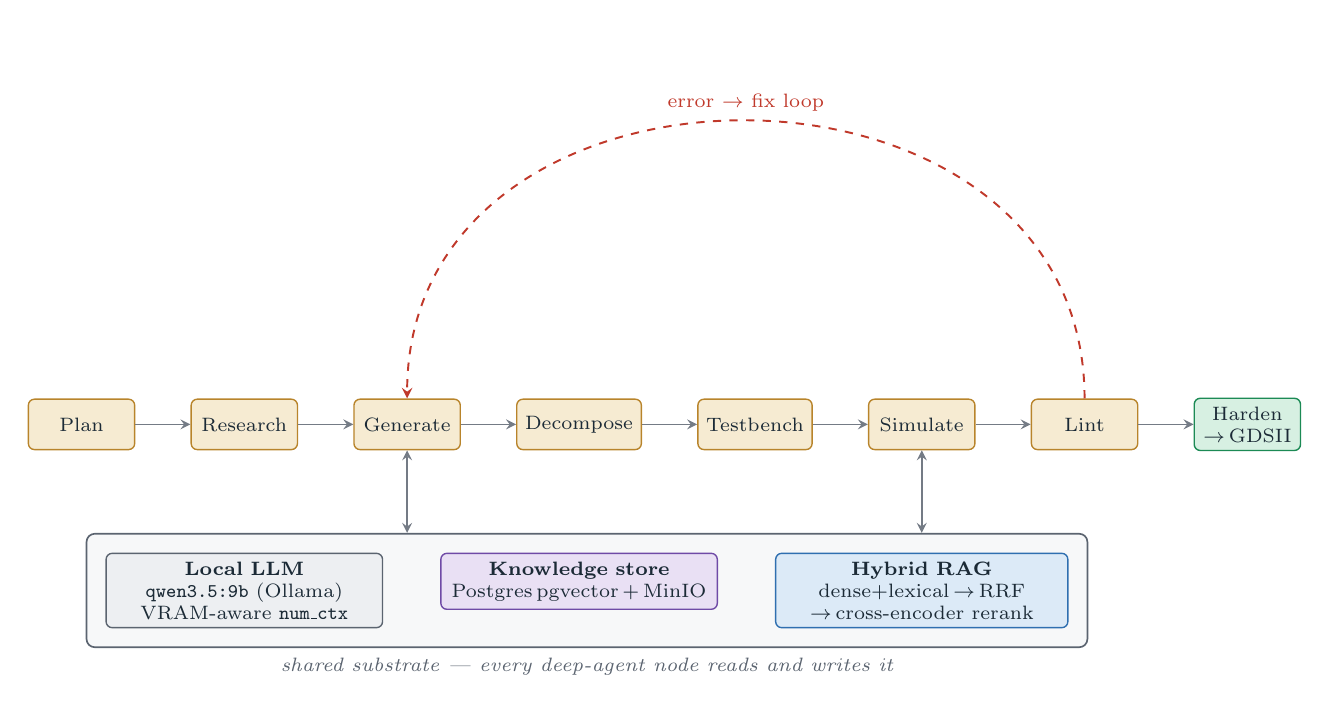
\begin{tikzpicture}[node distance=6mm and 7mm]
  % --- pipeline band ---
  \node[stage](plan){Plan};
  \node[stage,right=of plan](res){Research};
  \node[stage,right=of res](gen){Generate};
  \node[stage,right=of gen](dec){Decompose};
  \node[stage,right=of dec](tb){Testbench};
  \node[stage,right=of tb](sim){Simulate};
  \node[stage,right=of sim](lint){Lint};
  \node[hard,right=of lint](hard){Harden\\$\to$\,GDSII};
  \foreach \a/\b in {plan/res,res/gen,gen/dec,dec/tb,tb/sim,sim/lint,lint/hard}
     \draw[flow](\a)--(\b);
  % error->fix feedback arc (tidy, above the band)
  \draw[fb] (lint.north) to[out=90,in=90,looseness=1.4]
        node[pos=0.5,above,lbl,text=rred,font=\scriptsize]{error $\to$ fix loop} (gen.north);
  % --- shared substrate, evenly under the band ---
  \node[nn, below=13mm of res, text width=33mm]
       (llm){\textbf{Local LLM}\\\texttt{qwen3.5:9b} (Ollama)\\VRAM-aware \texttt{num\_ctx}};
  \node[pp, below=13mm of dec, text width=33mm]
       (ks){\textbf{Knowledge store}\\Postgres\,pgvector\,+\,MinIO};
  \node[bb, below=13mm of sim, text width=35mm]
       (rag){\textbf{Hybrid RAG}\\dense+lexical\,$\to$\,RRF\\$\to$\,cross-encoder rerank};
  \begin{scope}[on background layer]
    \node[grp=gry, fill=gryL!45, fit=(llm)(ks)(rag),
          label={[lbl,gry,font=\scriptsize]below:\itshape shared substrate --- every deep-agent node reads and writes it}](sub){};
  \end{scope}
  \draw[flowt] (gen) -- (gen|-sub.north);
  \draw[flowt] (sim) -- (sim|-sub.north);
\end{tikzpicture}}
\caption{GarudaChip architecture. A fixed, deterministic pipeline graph (top) drives the
prompt-to-GDSII flow with an error-to-fix feedback loop; each reasoning node executes as an
RLM deep agent (Fig.~\ref{fig:rlm}) over a shared substrate (bottom): a local model with a
VRAM-aware context window, a durable knowledge store, and a hybrid retrieval stack.}
\label{fig:arch}
\end{figure*}

\section{Introduction}
The cost and scarcity of digital-design expertise motivate tools that lower the
barrier from intent to silicon. Recent LLMs can draft Verilog, but production use
in defense and sovereign-technology settings raises two hard constraints: design
data must never leave the premises, and the available compute is modest. Cloud
LLM APIs violate the first; large local models violate the second. GarudaChip
targets exactly this regime: a single workstation, an open-source toolchain, and
a small local model.

Our central claim is that a small local model becomes a capable hardware designer
when it is embedded in the right scaffolding: a deterministic flow graph that
guarantees the right step runs at the right time; deep agents that plan and use
tools instead of emitting code in one shot; a knowledge base that remembers every
prior design, reference and verified fix; and a retrieval pipeline good enough
that the few thousand tokens the model can attend to are the most relevant ones
available. Fig.~\ref{fig:arch} gives the overview; we then detail the deep-agent
node (Fig.~\ref{fig:rlm}), the autoresearch loop (Fig.~\ref{fig:auto}), the
deep-agent roster (Fig.~\ref{fig:roster}), and hybrid RAG (Fig.~\ref{fig:rag}),
before reporting case-study results.

\section{Related Work}
LLM-assisted RTL design has been explored by domain-adapted models such as
ChipNeMo~\cite{chipnemo} and by benchmarks like VerilogEval~\cite{verilogeval}
and RTLLM~\cite{rtllm}, which mostly evaluate single-shot code generation.
Agentic methods add planning and tool use; Reflexion-style self-improvement
loops~\cite{reflexion} let an agent learn from execution feedback. Recursive
language models~\cite{rlm} decompose a task so a model interacts with an external
context it never fully loads. On the retrieval side, RAG~\cite{rag} augments
generation with fetched context; hybrid search and reciprocal rank fusion
(RRF)~\cite{rrf} combine dense and lexical rankings, and cross-encoder
rerankers~\cite{sbert} sharply improve precision. GarudaChip integrates these
threads into an end-to-end, local prompt-to-GDSII flow with an open-source
hardening back end (LibreLane/OpenROAD~\cite{openroad,librelane} on
GF180MCU~\cite{gf180}).

\section{System Architecture}
GarudaChip is a fixed directed graph of pipeline stages (Fig.~\ref{fig:arch}).
The graph is deterministic: it always plans before it generates and always
simulates and lints before it hardens, with an error-to-fix arc that returns
failing designs to generation. Determinism at the graph level supplies the
guardrails a small model needs; flexibility lives inside each node.

% ===================== FIG 2: RLM deep agent (single col) ==================
\begin{figure}[t]
\centering
\resizebox{\columnwidth}{!}{%
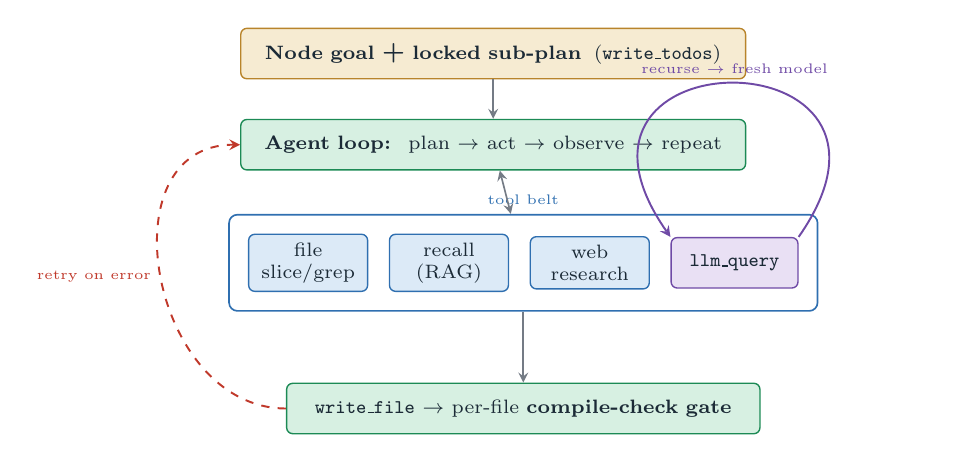
\begin{tikzpicture}[node distance=5mm]
  \node[yy, text width=62mm](goal){\textbf{Node goal {\small+} locked sub-plan}\;\;(\texttt{write\_todos})};
  \node[gg, below=of goal, text width=62mm](loop){\textbf{Agent loop:}\; plan $\to$ act $\to$ observe $\to$ repeat};
  % tool belt
  \node[bb, below=8mm of loop.south, anchor=north, xshift=-23.5mm, text width=13mm](t1){file\\slice/grep};
  \node[bb, right=2.6mm of t1, text width=13mm](t2){recall\\(RAG)};
  \node[bb, right=2.6mm of t2, text width=13mm](t3){web\\research};
  \node[pp, right=2.6mm of t3, text width=14mm](t4){\texttt{llm\_query}};
  \begin{scope}[on background layer]
    \node[grp=blu, fit=(t1)(t2)(t3)(t4), label={[lbl,blu]above:tool belt}](belt){};
  \end{scope}
  \node[hard, below=9mm of belt.south, text width=58mm]
       (gate){\texttt{write\_file} $\to$ per-file \textbf{compile-check gate}};
  \draw[flow](goal)--(loop);
  \draw[flowt](loop)--(belt);
  \draw[flow](belt)--(gate);
  % recursion: self-loop on llm_query
  \draw[rec] (t4.north east) to[out=55,in=125,looseness=5]
        node[above,lbl,text=pur]{recurse $\to$ fresh model} (t4.north west);
  % retry on compile error, routed on the left
  \draw[fb] (gate.west) to[out=180,in=180,looseness=1.3]
        node[left,lbl,text=rred]{retry on error} (loop.west);
\end{tikzpicture}}
\caption{Anatomy of one RLM deep agent. A node plans a to-do list, then loops over a shared
tool belt---file slicing, RAG recall, web research, and \texttt{llm\_query}, the recursive
leaf that delegates a focused sub-task to a fresh model instance. Every file write passes a
compile-check gate before the node may finish.}
\label{fig:rlm}
\end{figure}

\subsection{Deep agents per node}
Each reasoning stage---planner, researcher, generator, testbench writer, and the
module and testbench correctors---executes as a deep agent
(Fig.~\ref{fig:rlm}): it writes a to-do list, reads and greps files in slices
rather than swallowing them, issues focused recursive sub-calls
(\texttt{llm\_query}) to a fresh model instance, and can search the web.
Mechanical stages (decompose, write, simulate, lint, harden) are deliberately
kept free of the LLM and run regex/Icarus/Verilator/LibreLane so generated code
is preserved byte-for-byte. Fig.~\ref{fig:roster} lists the agent roster.

\subsection{Durable knowledge store}
Long-term memory is a Postgres database with the pgvector extension for
embeddings and a MinIO object store for raw artifacts---RTL, references, papers,
waveforms and GDS. Every finished design is ingested, so the system improves with
use; a committed seed ships with the repository so a fresh clone is never empty.
The store is defensive: if it is unavailable the agent falls back to a
pure-local file flow.

\subsection{Local model and context window}
All generation uses a local Ollama-served \texttt{qwen3.5:9b} model. Because the
key--value cache of such a model costs on the order of 56\,KB per token, the
usable context window is bounded by GPU memory, not by the model. GarudaChip
detects the available VRAM (or system RAM under CPU inference) and exposes a
context-window slider whose maximum is the key--value-cache budget after
reserving the model weights, so a user can trade context for memory and never
select a window that will not fit.

% ===================== FIG 3: autoresearch loop (single col) ==============
\begin{figure}[t]
\centering
\resizebox{\columnwidth}{!}{%
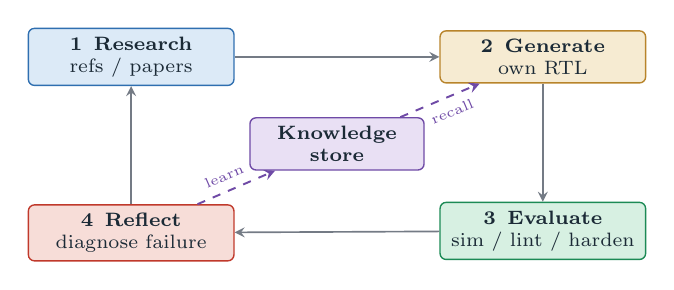
\begin{tikzpicture}[node distance=15mm and 26mm]
  \node[bb, text width=24mm](research){\textbf{1\, Research}\\refs / papers};
  \node[yy, right=of research, text width=24mm](generate){\textbf{2\, Generate}\\own RTL};
  \node[gg, below=of generate, text width=24mm](evaluate){\textbf{3\, Evaluate}\\sim / lint / harden};
  \node[box, fill=rredL, draw=rred, below=of research, text width=24mm](reflect){\textbf{4\, Reflect}\\diagnose failure};
  \node[pp] at ($(research)!0.5!(evaluate)$) [text width=20mm](store){\textbf{Knowledge}\\\textbf{store}};
  \draw[flow](research)--(generate);
  \draw[flow](generate)--(evaluate);
  \draw[flow](evaluate)--(reflect);
  \draw[flow](reflect)--(research);
  \draw[rec, dashed](reflect) -- (store) node[pos=0.42,above,sloped,lbl,text=pur]{learn};
  \draw[rec, dashed](store) -- (generate) node[pos=0.58,below,sloped,lbl,text=pur]{recall};
\end{tikzpicture}}
\caption{Autoresearch self-improvement loop. The agent researches references, authors RTL,
evaluates it with the open-source tools, and reflects on failures; verified error-to-fix
lessons and generation methods are written to the knowledge store and recalled on the next
run, so quality compounds over time.}
\label{fig:auto}
\end{figure}

\section{Generate-From-Knowledge, Autoresearch, and Hybrid RAG}
A naive agent that clones the nearest reference repository produces designs that
are merely renamed copies, sometimes hundreds of near-identical blocks.
GarudaChip instead treats retrieved repositories and papers as knowledge to
study, not code to paste. The architect derives its own module map and is
instructed to collapse repetition into one parameterized module instantiated $N$
times; the generator then authors each module itself, grounded in retrieved
knowledge and guarded by per-file compile checks and a completeness gate.

\subsection{Autoresearch}
GarudaChip closes a self-improvement loop (Fig.~\ref{fig:auto}). After each run,
verified error-to-fix pairs and effective generation methods are written to the
knowledge store; on subsequent runs they are recalled and injected before
generation, so the agent stops repeating past mistakes. This Reflexion-style loop
turns the durable store into accumulating expertise rather than a static index.

\subsection{Deep-agent roster}
Fig.~\ref{fig:roster} summarizes the specialized agents. They share the same tool
belt and substrate but differ in goal and in which tools dominate: the researcher
leans on web search and crawling, the generator on knowledge recall and the
compile-check gate, and the correctors on error-grounded retrieval.

% ===================== FIG 4: deep-agent roster (single col) ==============
\begin{figure}[t]
\centering
\resizebox{\columnwidth}{!}{%
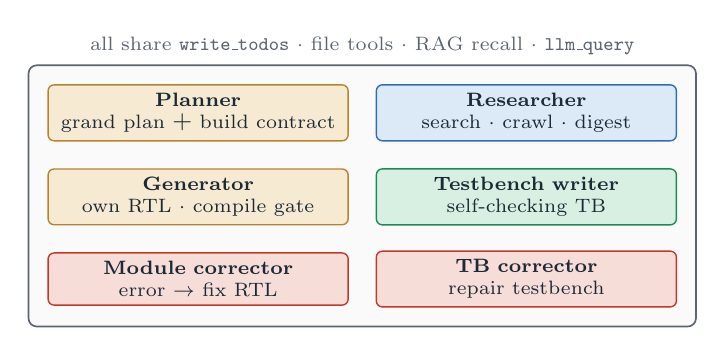
\begin{tikzpicture}[node distance=3.4mm and 3.4mm]
  \node[yy, text width=36mm](pl){\textbf{Planner}\\grand plan {\small+} build contract};
  \node[bb, right=of pl, text width=36mm](rs){\textbf{Researcher}\\search $\cdot$ crawl $\cdot$ digest};
  \node[yy, below=of pl, text width=36mm](ge){\textbf{Generator}\\own RTL $\cdot$ compile gate};
  \node[gg, right=of ge, text width=36mm](tw){\textbf{Testbench writer}\\self-checking TB};
  \node[box,fill=rredL,draw=rred, below=of ge, text width=36mm](mc){\textbf{Module corrector}\\error $\to$ fix RTL};
  \node[box,fill=rredL,draw=rred, right=of mc, text width=36mm](tc){\textbf{TB corrector}\\repair testbench};
  \begin{scope}[on background layer]
    \node[grp=gry, fill=gryL!30, fit=(pl)(rs)(ge)(tw)(mc)(tc),
          label={[lbl,gry,font=\scriptsize]above:all share \texttt{write\_todos} $\cdot$ file tools $\cdot$ RAG recall $\cdot$ \texttt{llm\_query}}]{};
  \end{scope}
\end{tikzpicture}}
\caption{The deep-agent roster. Each pipeline node is a specialized agent with its own goal,
drawing on a common tool belt; LLM-free stages (decompose, write, simulate, lint, harden)
are omitted.}
\label{fig:roster}
\end{figure}

\subsection{Hybrid retrieval}
Under a tight context budget, retrieval quality is decisive. Recall is hybrid
(Fig.~\ref{fig:rag}): a dense pgvector cosine search and a lexical Postgres
full-text search are each run broadly, merged by reciprocal rank fusion, and then
reranked by a local cross-encoder that scores every query--passage pair jointly.
Only the few highest-scoring chunks enter the prompt, maximizing signal per
token. Each stage degrades gracefully: without the full-text index the system is
dense-only, and without the reranker it falls back to fusion order.

% ===================== FIG 5: hybrid RAG (single col) =====================
\begin{figure}[t]
\centering
\resizebox{\columnwidth}{!}{%
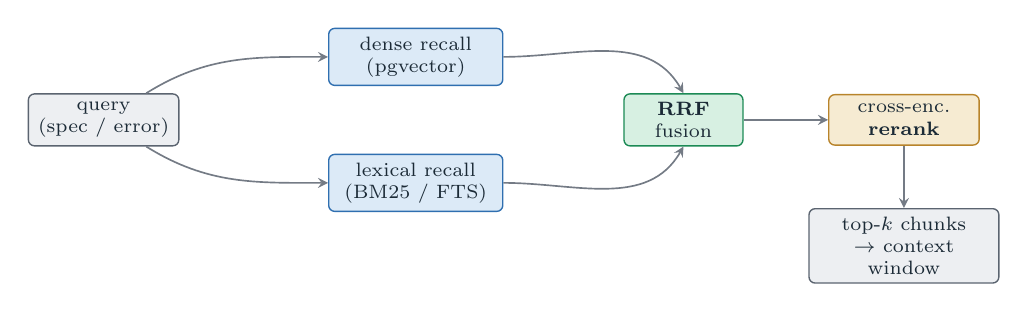
\begin{tikzpicture}
  \node[nn, text width=17mm](q){query\\(spec / error)};
  \node[bb, text width=20mm](dense) at ([xshift=30mm,yshift=8mm]q.east){dense recall\\(pgvector)};
  \node[bb, text width=20mm](lex)   at ([xshift=30mm,yshift=-8mm]q.east){lexical recall\\(BM25 / FTS)};
  \node[gg, text width=13mm](rrf)   at ([xshift=64mm]q.east){\textbf{RRF}\\fusion};
  \node[yy, text width=17mm](rk)    at ([xshift=92mm]q.east){cross-enc.\\\textbf{rerank}};
  \node[nn, text width=22mm](top)   at ([yshift=-16mm]rk){top-$k$ chunks\\$\to$ context window};
  \draw[flow](q) to[out=32,in=180] (dense.west);
  \draw[flow](q) to[out=-32,in=180] (lex.west);
  \draw[flow](dense.east) to[out=0,in=120] (rrf.north);
  \draw[flow](lex.east) to[out=0,in=240] (rrf.south);
  \draw[flow](rrf)--(rk);
  \draw[flow](rk)--(top);
\end{tikzpicture}}
\caption{Hybrid retrieval: dense and lexical recall are fused by RRF, reranked by a local
cross-encoder, and only the top-$k$ chunks are sent to the model.}
\label{fig:rag}
\end{figure}

As a qualitative check, for the query ``8-bit ALU with carry flag'' the
cross-encoder scored a matching ALU passage far above an unrelated UART passage,
and hybrid recall returned ALU register-transfer code and design notes ahead of
weaker matches, confirming that the reranker reorders fused candidates by true
relevance.

\section{Results}
We report two case studies produced end-to-end by the system and summarized in
Table~\ref{tab:results}. The knowledge store currently holds 1{,}125 indexed
items (700 code, 206 reusable IP, 63 GDS, 49 verified fixes, 23 papers and
others), and the bundled IP library exposes 92 blocks spanning CPU cores,
memories, buses, peripherals, DSP and cryptography.

\begin{table}[t]
\caption{End-to-end case-study results on the open-source GF180MCU flow.}
\label{tab:results}
\centering
\renewcommand{\arraystretch}{1.15}
\begin{tabular}{lll}
\toprule
\textbf{Metric} & \textbf{FazyRV RV32I} & \textbf{CGRA 2$\times$2} \\
\midrule
RTL files / lines      & 23 / 4332        & multi / param. \\
RTL simulation         & PASS             & PASS \\
Synthesis (Yosys)      & clean            & 0 err / 0 warn \\
GDSII (GF180MCU)       & produced         & RTL + synth. \\
Die area               & 5304\,$\mu$m$^2$ & --- \\
Placed instances       & 207              & --- \\
Lint errors            & 0                & 0 \\
Setup/hold violations  & 0 (tt/ss/ff)     & --- \\
\bottomrule
\end{tabular}
\end{table}

\subsection{RV32I soft core}
From the prompt ``create a FazyRV 8-bit RISC-V'', GarudaChip produced a 23-file,
4{,}332-line RTL core that passes self-checking simulation and hardens to GDSII
on GF180MCU. Static timing analysis reported zero setup and zero hold violations
across the typical, slow and fast corners (\textit{nom\_tt}
25\,\textcelsius/5.0\,V, \textit{nom\_ss} 125\,\textcelsius/4.5\,V,
\textit{nom\_ff} $-$40\,\textcelsius/5.5\,V); the layout has a die area of
5304\,$\mu$m$^2$ with 207 placed instances and no lint errors---a clean,
sign-off-ready macro.

\subsection{Coarse-grained reconfigurable array}
A 2$\times$2 CGRA accelerator exercises the parameterized
generate-from-knowledge path: a processing-element tile is described once and
instantiated across the array rather than emitted as repeated copies. The design
passes simulation and synthesizes cleanly in Yosys with zero errors and zero
warnings, providing the netlist for subsequent placement and routing.

\section{Discussion and Limitations}
GarudaChip shows that scaffolding, not model scale, is the lever for local
agentic EDA: a 9B model with hybrid reranked retrieval and a deterministic flow
reaches GDSII sign-off on a real PDK. Limitations remain. Throughput is bounded
by local inference, so complex designs require several generate--verify
iterations; the current evaluation is case-study rather than a large benchmark
sweep; and hardening is validated on GF180MCU only. The reranker adds a one-time
model download and a small per-query cost. Future work includes a quantitative
VerilogEval/RTLLM comparison, contextual-retrieval chunk augmentation at
ingestion, and power- and area-directed optimization loops.

\section{Conclusion}
We presented GarudaChip, a fully local recursive-language-model agent that
converts natural-language intent into RTL and GDSII on an open-source toolchain.
By combining a deterministic pipeline of deep agents, an autoresearch
self-improvement loop, a durable knowledge store, hybrid reranked retrieval and a
VRAM-aware context window, the system makes a small on-premises model a practical
hardware designer, achieving a clean multi-corner sign-off for an RV32I core and
simulation-plus-synthesis closure for a reconfigurable accelerator.

\section*{Acknowledgment}
The author thanks Pindad Military Ltd.\ for supporting sovereign, on-premises
design-automation research. GarudaChip builds on open-source projects including
Ollama, pgvector, MinIO, Yosys, OpenROAD, LibreLane and the GF180MCU PDK.

\begin{thebibliography}{99}
\bibitem{chipnemo} M.~Liu \textit{et al.}, ``ChipNeMo: Domain-adapted LLMs for
chip design,'' arXiv:2311.00176, 2023.
\bibitem{verilogeval} M.~Liu \textit{et al.}, ``VerilogEval: Evaluating large
language models for Verilog code generation,'' in \textit{Proc. ICCAD}, 2023.
\bibitem{rtllm} Y.~Lu \textit{et al.}, ``RTLLM: An open-source benchmark for
design RTL generation with large language models,'' in \textit{Proc. ASP-DAC},
2024.
\bibitem{reflexion} N.~Shinn \textit{et al.}, ``Reflexion: Language agents with
verbal reinforcement learning,'' in \textit{Proc. NeurIPS}, 2023.
\bibitem{rlm} MIT CSAIL, ``Recursive Language Models,'' arXiv preprint, 2025.
\bibitem{rag} P.~Lewis \textit{et al.}, ``Retrieval-augmented generation for
knowledge-intensive NLP tasks,'' in \textit{Proc. NeurIPS}, 2020.
\bibitem{rrf} G.~V.~Cormack, C.~L.~A.~Clarke, and S.~Buettcher, ``Reciprocal
rank fusion outperforms Condorcet and individual rank learning methods,'' in
\textit{Proc. SIGIR}, 2009.
\bibitem{sbert} N.~Reimers and I.~Gurevych, ``Sentence-BERT: Sentence embeddings
using Siamese BERT-networks,'' in \textit{Proc. EMNLP}, 2019.
\bibitem{qwen} A.~Yang \textit{et al.}, ``Qwen technical report,''
arXiv:2412.15115, 2024.
\bibitem{yosys} C.~Wolf, ``Yosys open synthesis suite,''
\url{https://yosyshq.net}, 2023.
\bibitem{openroad} T.~Ajayi \textit{et al.}, ``OpenROAD: Toward a self-driving,
open-source digital layout implementation tool chain,'' in \textit{Proc.
GOMACTech}, 2019.
\bibitem{librelane} Efabless and contributors, ``LibreLane / OpenLane
RTL-to-GDSII flow,'' 2024.
\bibitem{gf180} GlobalFoundries and Google, ``GF180MCU open-source PDK,'' 2022.
\end{thebibliography}

\end{document}
